\documentclass[12pt]{article}

\usepackage[english]{babel}
\usepackage[utf8]{inputenc}
\usepackage{sansmathfonts}
\usepackage[T1]{fontenc}
\renewcommand*\familydefault{\sfdefault} %% Only if the base font of the document is to be sans serif
\usepackage{multicol,lipsum}
\usepackage{amsmath,cancel}
\usepackage{amssymb,amsthm,dsfont,mathrsfs}
\usepackage[colorinlistoftodos]{todonotes}
\usepackage{geometry}
\geometry{
a4paper,
total={170mm,257mm},
left=20mm,
top=15mm,
bottom=22mm,
}
\usepackage{natbib}
\usepackage{soul}
\usepackage{setspace}
\usepackage{hyperref}
\usepackage{xcolor}
\usepackage{graphicx}
\usepackage{tikz}
\usepackage{siunitx}
\graphicspath{ {imagens/} }
\usepackage{fancyhdr}
\pagestyle{fancy}
\renewcommand{\headrulewidth}{0pt}

\color{darkgray}
\newcommand{\T}[1]{\vspace{0.4cm}\textbf{\large#1}}
\newcommand{\TW}[1]{\textbf{\large#1}}

\newcommand{\TM}[1]{\vspace{0.2cm} \textbf{#1}}

\newcommand{\M}[1]{
\vspace{-0.6cm}
\begin{flalign*}
#1&
\end{flalign*}
\vspace{-0.6cm}
}


\definecolor{bluebell}{rgb}{0.25, 0.35, 0.89} 
\definecolor{laranja}{rgb}{0.87, 0.48, 0.25} 
\definecolor{verde}{rgb}{0, 0.54, 0.44} 
\definecolor{babypink}{rgb}{1, 0.42, 0.52} 
\definecolor{rosa}{rgb}{1, 0.72, 0.77} 
\definecolor{cinza}{rgb}{0.3, 0.3, 0.3}  
\definecolor{iris}{rgb}{0.25, 0.35, 0.89}  
\definecolor{babyblue}{rgb}{0.13, 0.59, 0.95}

\setlength\columnsep{30pt}

\setlength{\parindent}{0cm}
\setlength{\fboxrule}{1.3pt}  % <-- Aumenta a espessura

\newcommand{\Formula}[1]{
\begin{center}
\color{iris}
\fcolorbox{rosa}{white}{
\(
\begin{array}{c}
#1
\end{array}
\)
}
\color{cinza}
\end{center}
}

\begin{document}
\pagenumbering{gobble}
\setstretch{1.3}


\includegraphics[width=4cm]{Logo2.png}
\begin{center}
    \textbf{\Huge \textcolor{bluebell}{Semelhança de Triângulos}}
\end{center}

\begin{multicols}{2}

% ── DEFINIÇÃO ──────────────────────────────────────────────────────────────
\TW{Definição}

Dois triângulos são semelhantes quando possuem ângulos correspondentes iguais e lados correspondentes proporcionais.

Dizemos que $\triangle ABC \sim \triangle A'B'C'$ (lê-se \textit{semelhante}) quando existe um valor $k$ — chamado de \textbf{razão de semelhança} — tal que:

\Formula{
\dfrac{AB}{A'B'} = \dfrac{BC}{B'C'} = \dfrac{AC}{A'C'} = k
}

Se $k = 1$ os triângulos são congruentes; se $k \neq 1$ são semelhantes mas de tamanhos diferentes.

\vspace{0.2cm}
\fcolorbox{laranja}{white}{\parbox{0.85\linewidth}{
\small\textbf{Atenção — ordem dos vértices:} a notação $ABC \sim A'B'C'$ exige correspondência posicional: $A \leftrightarrow A'$, $B \leftrightarrow B'$, $C \leftrightarrow C'$. Inverter a ordem invalida a proporção.
}}
\vspace{0.2cm}

% ── TEOREMA DE TALES ───────────────────────────────────────────────────────
\TW{Teorema de Tales}

Se duas retas transversais cortam um feixe de retas paralelas, os segmentos determinados em uma transversal são proporcionais aos segmentos correspondentes na outra transversal.

\Formula{
\dfrac{\alpha}{\beta}  = \dfrac{\gamma}{\phi}
}

\begin{center}
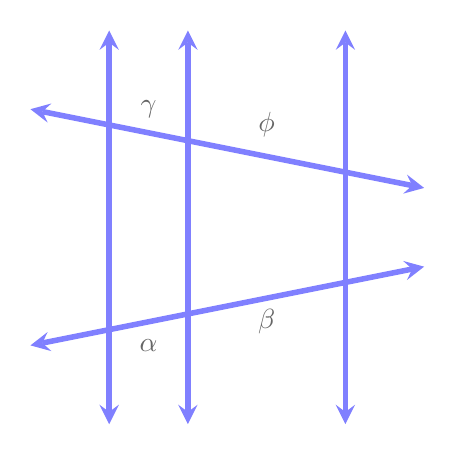
\begin{tikzpicture}
\tikzstyle{texto}=[draw=none,fill=none,black!60!white]
\tikzstyle{line}=[blue!50!white,line width=2pt]

\draw[line,stealth-stealth] (0,0) -- (5,1);
\draw[line,stealth-stealth] (0,3) -- (5,2);
\draw[line,stealth-stealth] (1,-1) -- (1,4);
\draw[line,stealth-stealth] (2,-1) -- (2,4);
\draw[line,stealth-stealth] (4,-1) -- (4,4);

\node[texto] at (1.5,0) {\textbf{$\alpha$}};
\node[texto] at (3,0.3) {\textbf{$\beta$}};
\node[texto] at (1.5,3) {\textbf{$\gamma$}};
\node[texto] at (3,2.8) {\textbf{$\phi$}};
\end{tikzpicture}
\end{center}

A proporção se mantém ao substituir um segmento pela soma de segmentos adjacentes:

\Formula{
\dfrac{\alpha+\beta}{\beta}  = \dfrac{\gamma+\phi}{\phi}
\qquad\text{e}\qquad
\dfrac{\alpha}{\alpha + \beta}  = \dfrac{\gamma}{\gamma + \phi}
}

\TM{Exemplos — Teorema de Tales:}

\begin{center}
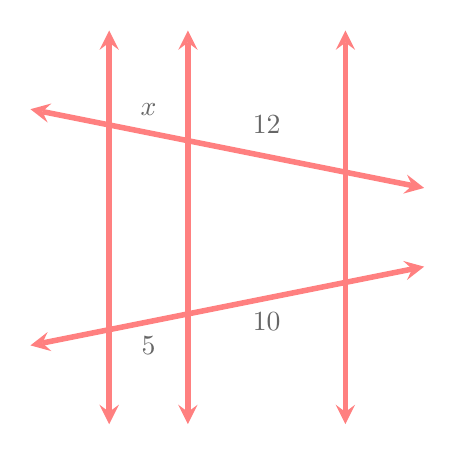
\begin{tikzpicture}
\tikzstyle{texto}=[draw=none,fill=none,black!60!white]
\tikzstyle{line}=[red!50!white,line width=2pt]

\draw[line,stealth-stealth] (0,0) -- (5,1);
\draw[line,stealth-stealth] (0,3) -- (5,2);
\draw[line,stealth-stealth] (1,-1) -- (1,4);
\draw[line,stealth-stealth] (2,-1) -- (2,4);
\draw[line,stealth-stealth] (4,-1) -- (4,4);

\node[texto] at (1.5,0) {\textbf{$5$}};
\node[texto] at (3,0.3) {\textbf{$10$}};
\node[texto] at (1.5,3) {\textbf{$x$}};
\node[texto] at (3,2.8) {\textbf{$12$}};
\end{tikzpicture}
\end{center}

\vspace{4pt}
$\dfrac{5}{10} = \dfrac{x}{12}$\vspace{6pt}

$\dfrac{x}{12} = \dfrac{1}{2}$\vspace{6pt}

$x = \dfrac{1}{2} \cdot 12$\vspace{6pt}

$\boxed{x = 6}$

\vspace{0.3cm}
Dados $\alpha = 3$, $\beta = 9$, $\gamma = 2$ e $\phi = x$:\vspace{4pt}

$\dfrac{3}{9} = \dfrac{2}{x} \Rightarrow 3x = 18$\vspace{6pt}

$\boxed{x = 6}$

% ── CRITÉRIO AA ────────────────────────────────────────────────────────────
\TW{Critério AA — Ângulo-Ângulo}

Se dois triângulos possuem dois ângulos correspondentes iguais, então são semelhantes e possuem lados proporcionais.

\begin{center}
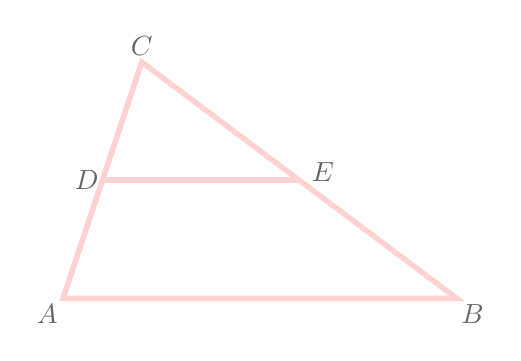
\begin{tikzpicture}
\tikzstyle{texto}=[draw=none,fill=none,black!60!white]
\tikzstyle{line}=[pink!70!white,line width=2pt]

\draw[line] (0,0) -- (5,0) -- (1,3) -- cycle;
\draw[line] (0.5,1.5) -- (3,1.5);

\node[texto] at (-0.2,-0.2) {\textbf{$A$}};
\node[texto] at (5.2,-0.2) {\textbf{$B$}};
\node[texto] at (1,3.2) {\textbf{$C$}};
\node[texto] at (0.3,1.5) {\textbf{$D$}};
\node[texto] at (3.3,1.6) {\textbf{$E$}};
\end{tikzpicture}
\end{center}

$DE \parallel AB \Rightarrow \angle CDE = \angle CAB$ e $\angle CED = \angle CBA$

Logo $\triangle CDE \sim \triangle CAB$ e:

\Formula{
\dfrac{CD}{CA} = \dfrac{CE}{CB} = \dfrac{DE}{AB}
}

% ── CRITÉRIO LAL ───────────────────────────────────────────────────────────
\TW{Critério LAL — Lado-Ângulo-Lado}

Dois triângulos são semelhantes quando dois pares de lados correspondentes são proporcionais e os ângulos entre esses lados são iguais.

\TM{Exemplo:}

$\triangle ABC$: $AB = 4$, $AC = 6$, $\angle A = 50°$

$\triangle DEF$: $DE = 8$, $DF = 12$, $\angle D = 50°$\vspace{4pt}

$\dfrac{AB}{DE} = \dfrac{4}{8} = \dfrac{1}{2}$ \quad e \quad $\dfrac{AC}{DF} = \dfrac{6}{12} = \dfrac{1}{2}$\vspace{6pt}

Razões iguais e ângulo incluído igual:

$\boxed{\triangle ABC \sim \triangle DEF \text{ (LAL)}, \; k = 2}$

% ── CRITÉRIO LLL ───────────────────────────────────────────────────────────
\TW{Critério LLL — Lado-Lado-Lado}

Dois triângulos são semelhantes quando os três pares de lados correspondentes são proporcionais, com um único valor $k$.

\TM{Exemplo:}

$\triangle ABC$: lados $3$, $4$ e $6$

$\triangle DEF$: lados $6$, $8$ e $12$\vspace{4pt}

$\dfrac{3}{6} = \dfrac{4}{8} = \dfrac{6}{12} = \dfrac{1}{2}$\vspace{6pt}

$\boxed{\triangle ABC \sim \triangle DEF \text{ (LLL)}, \; k = 2}$

% ── PROPRIEDADES ───────────────────────────────────────────────────────────
\TW{Propriedades dos Triângulos Semelhantes}

Se $\triangle ABC \sim \triangle A'B'C'$ com razão de semelhança $k$:

\Formula{
\dfrac{P}{P'} = k \qquad \dfrac{A}{A'} = k^2 \qquad \dfrac{h}{h'} = k \qquad \dfrac{m}{m'} = k
}

Onde $P$ = perímetro, $A$ = área, $h$ = altura correspondente e $m$ = mediana correspondente. As alturas e medianas crescem na mesma proporção dos lados; a área cresce com o \textbf{quadrado} da razão.

\TM{Exemplos:}

Dois triângulos semelhantes com $k = 3$; menor tem área $10\,\text{cm}^2$:\vspace{4pt}

$A' = 10 \cdot 3^2 = 10 \cdot 9 = \boxed{90\,\text{cm}^2}$\vspace{6pt}

Perímetro do menor é $12\,\text{cm}$ e $k = 2$:\vspace{4pt}

$P' = 12 \cdot 2 = \boxed{24\,\text{cm}}$

% ── EXEMPLOS RESOLVIDOS ────────────────────────────────────────────────────
\TW{Exemplos Resolvidos}

\TM{Exemplo 1 — Tales com triângulo ($CD=4$, $DE=6$, $AB=12$, $DA=x$):}

\begin{center}
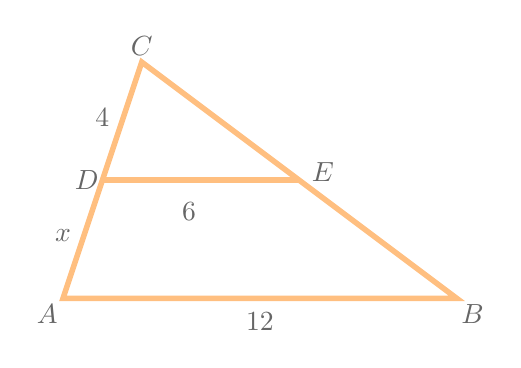
\begin{tikzpicture}
\tikzstyle{texto}=[draw=none,fill=none,black!60!white]
\tikzstyle{line}=[orange!50!white,line width=2pt]

\draw[line] (0,0) -- (5,0) -- (1,3) -- cycle;
\draw[line] (0.5,1.5) -- (3,1.5);

\node[texto] at (2.5,-0.3) {\textbf{$12$}};
\node[texto] at (1.6,1.1) {\textbf{$6$}};
\node[texto] at (0.5,2.3) {\textbf{$4$}};
\node[texto] at (0,0.8) {\textbf{$x$}};

\node[texto] at (-0.2,-0.2) {\textbf{$A$}};
\node[texto] at (5.2,-0.2) {\textbf{$B$}};
\node[texto] at (1,3.2) {\textbf{$C$}};
\node[texto] at (0.3,1.5) {\textbf{$D$}};
\node[texto] at (3.3,1.6) {\textbf{$E$}};
\end{tikzpicture}
\end{center}

\vspace{4pt}
$\dfrac{CD}{CA} = \dfrac{DE}{AB} \Rightarrow \dfrac{4}{4+x} = \dfrac{6}{12} = \dfrac{1}{2}$\vspace{6pt}

$4 \cdot 2 = 4 + x \Rightarrow 8 = 4 + x$\vspace{6pt}

$\boxed{x = 4}$

\vspace{0.3cm}
\TM{Exemplo 2 — Proporcionalidade ($CD=4$, $DA=6$, $CE=8$, $EB=x$):}

\begin{center}
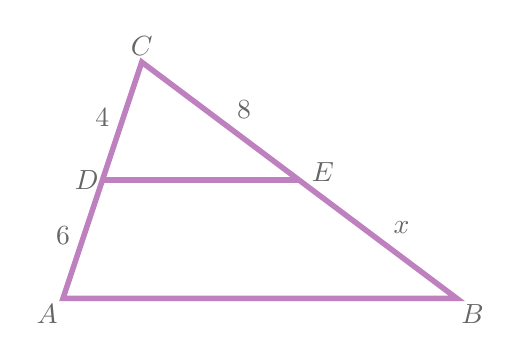
\begin{tikzpicture}
\tikzstyle{texto}=[draw=none,fill=none,black!60!white]
\tikzstyle{line}=[violet!50!white,line width=2pt]

\draw[line] (0,0) -- (5,0) -- (1,3) -- cycle;
\draw[line] (0.5,1.5) -- (3,1.5);

\node[texto] at (4.3,0.9) {\textbf{$x$}};
\node[texto] at (2.3,2.4) {\textbf{$8$}};
\node[texto] at (0.5,2.3) {\textbf{$4$}};
\node[texto] at (0,0.8) {\textbf{$6$}};

\node[texto] at (-0.2,-0.2) {\textbf{$A$}};
\node[texto] at (5.2,-0.2) {\textbf{$B$}};
\node[texto] at (1,3.2) {\textbf{$C$}};
\node[texto] at (0.3,1.5) {\textbf{$D$}};
\node[texto] at (3.3,1.6) {\textbf{$E$}};
\end{tikzpicture}
\end{center}

\vspace{4pt}
$\dfrac{CD}{DA} = \dfrac{CE}{EB} \Rightarrow \dfrac{4}{6} = \dfrac{8}{x}$\vspace{6pt}

$4x = 8 \cdot 6 = 48$\vspace{6pt}

$\boxed{x = 12}$

\vspace{0.3cm}
\TM{Exemplo 3 — Razão de semelhança (lados $4$, $6$, $8$; menor lado $= 6$):}

$k = \dfrac{6}{4} = \dfrac{3}{2}$\vspace{6pt}

Segundo lado: $6 \cdot \dfrac{3}{2} = \boxed{9}$\vspace{6pt}

Terceiro lado: $8 \cdot \dfrac{3}{2} = \boxed{12}$

% ── SEMELHANÇA EM TRIÂNGULOS RETÂNGULOS ────────────────────────────────────
\TW{Semelhança em Triângulos Retângulos}

Ao traçar a altura $h$ relativa à hipotenusa de um triângulo retângulo, formam-se \textbf{três triângulos semelhantes entre si}:

\Formula{
\triangle ABC \sim \triangle ACH \sim \triangle CBH
}

Sendo $m$ e $n$ as projeções dos catetos sobre a hipotenusa ($a = m + n$):

\Formula{
h^2 = m \cdot n \qquad b^2 = a \cdot m \qquad c^2 = a \cdot n
}

\TM{Exemplo ($b = 6$, $c = 8$; calcular $h$):}

$a = \sqrt{6^2 + 8^2} = \sqrt{100} = 10$\vspace{6pt}

$m = \dfrac{b^2}{a} = \dfrac{36}{10} = 3{,}6$ \quad $n = \dfrac{c^2}{a} = \dfrac{64}{10} = 6{,}4$\vspace{6pt}

$h^2 = 3{,}6 \times 6{,}4 = 23{,}04$\vspace{6pt}

$\boxed{h = 4{,}8}$

\vspace{0.1cm}
{\small\textit{Verificação: $a \cdot h = 10 \times 4{,}8 = 48 = b \cdot c = 6 \times 8$ \checkmark}}

% ── PROBLEMA CONTEXTUALIZADO ───────────────────────────────────────────────
\TW{Problema Contextualizado}

\TM{Problema 1 — Altura de uma árvore:}

Um poste de $2\,\text{m}$ projeta sombra de $3\,\text{m}$. Ao mesmo instante, uma árvore projeta sombra de $12\,\text{m}$. Qual é a altura da árvore?

\vspace{4pt}
Raios solares paralelos $\Rightarrow$ triângulos semelhantes (AA):\vspace{4pt}

$\dfrac{2}{h} = \dfrac{3}{12} \Rightarrow 3h = 24$\vspace{6pt}

$\boxed{h = 8\,\text{m}}$

\vspace{0.3cm}
\TM{Problema 2 — Largura de um rio:}

Pontos $C$, $D$, $E$ na margem, $DE \parallel AB$ (largura do rio), $CD = 10\,\text{m}$, $DA = 5\,\text{m}$, $DE = 8\,\text{m}$. Calcule $AB$.

\vspace{4pt}
$\triangle CDE \sim \triangle CAB$ (AA); $CA = 10 + 5 = 15\,\text{m}$\vspace{6pt}

$\dfrac{DE}{AB} = \dfrac{CD}{CA} \Rightarrow \dfrac{8}{AB} = \dfrac{10}{15} = \dfrac{2}{3}$\vspace{6pt}

$2 \cdot AB = 24$\vspace{6pt}

$\boxed{AB = 12\,\text{m}}$

\end{multicols}

\lfoot{\scriptsize © Copyright, Pratique Já}
\cfoot{\large \textcolor{bluebell}{pratiqueja.com}}
\end{document}
